\documentclass{beamer}
\usepackage[utf8]{inputenc}
\usepackage[]{amsmath}
\usepackage{graphicx}
\usepackage{physics}
\usepackage{subcaption} % package pour faire des subfigures
\usepackage{multirow} % package pour multirow/multicolumn
\usepackage{booktabs} % package pour top/mid/bottom rule
\usepackage{tcolorbox} % toujours plus de boites
\usepackage[backend=biber]{biblatex}


\addbibresource{Biblio_dbl_quantum.bib}

%\bibliographystyle{stylename}
%\bibliography{Biblio_dbl_quantum}

\title{QICS small seminar : NV center brief overview}
\author{Clément Pellet-Mary\\ LPENS, ENS Paris}
\date\today

\mode<presentation> {\usetheme{Rochester}}

\begin{document}
\begin{frame}
\maketitle
\centering
\includegraphics[scale=.5]{diamant_alex}
\includegraphics[scale=.2]{Nitrogen-vacancy_center}
\end{frame}
%\begin{frame}{Outline}
%\tableofcontents
%\end{frame}
%\section{Physics of the NV center}
\begin{frame}{Optical properties of NV$^-$ centers}
\centering
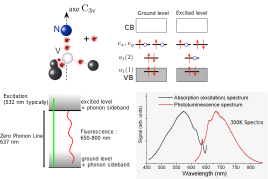
\includegraphics[width=\textwidth,height=0.9\textheight,keepaspectratio]{slide_NV_optical}
\end{frame}
\begin{frame}{NV$^-$ center electronic structure}
\centering
\includegraphics[width=\textwidth,height=0.9\textheight,keepaspectratio]{NV_8_niveaux_1}
\end{frame}
\begin{frame}{NV$^-$ center electronic structure}
\centering
\includegraphics[width=\textwidth,height=0.9\textheight,keepaspectratio]{NV_8_niveaux_2}
\end{frame}
\begin{frame}{NV$^-$ center electronic structure}
\centering
\includegraphics[width=\textwidth,height=0.9\textheight,keepaspectratio]{NV_8_niveaux_3}
\end{frame}
\begin{frame}{NV center spin sub-levels}
\centering
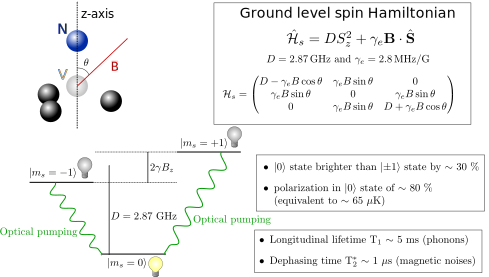
\includegraphics[width=\textwidth,height=0.9\textheight,keepaspectratio]{slide_3_niveaux}
\end{frame}
\begin{frame}{Practical example : Rabi oscillations}
\centering
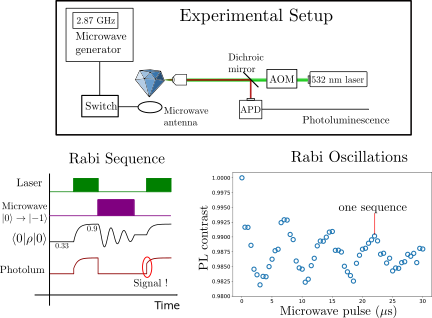
\includegraphics[width=\textwidth,height=0.9\textheight,keepaspectratio]{Slide_Rabi}
\end{frame}
\begin{frame}{Some NV successes}
\begin{itemize}
\item Quantum memory :
\includegraphics[width=\textwidth,height=0.9\textheight,keepaspectratio]{quantum_memory}
\item Intrication :
\includegraphics[width=0.8\textwidth,height=0.9\textheight,keepaspectratio]{intrication}
\item Quantum sensing (\underline{Magnetic field}, Electric field, Temperature) :
\includegraphics[width=\textwidth,height=0.9\textheight,keepaspectratio]{sensing}
\end{itemize}
\end{frame}
\begin{frame}{Our work}
\centering
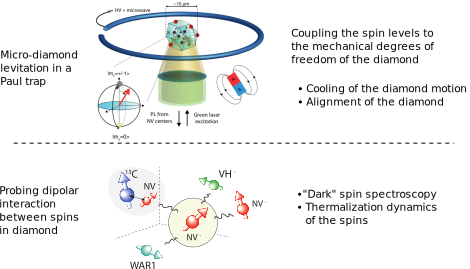
\includegraphics[width=\textwidth,height=0.9\textheight,keepaspectratio]{Slide our work}
\end{frame}


\end{document}